\documentclass[AMA,STIX2COL,Linenumbersoff]{MRM}

%% ----------
%%   Wiley
%% ----------

%%%%%%%%%%%%%%%%%%%%%%%%%%%%%%%%%%%%%%%%%%%%%%%%%%%%%%%
% A template for Wiley article submissions.
% Developed by Overleaf. 
%
% Please note that whilst this template provides a 
% preview of the typeset manuscript for submission, it 
% will not necessarily be the final publication layout.
%
% Usage notes:
% The "blind" option will make anonymous all author, affiliation, correspondence and funding information.
% Use "num-refs" option for numerical citation and references style.
% Use "alpha-refs" option for author-year citation and references style.

% Update article type if known
% \papertype{Note}
% Include section in journal if known, otherwise delete
% \paperfield{Submitted to Magnetic Resonance in Medicine}
\graphicspath{{./figures/}}

%% ---------------
%%   Word count
%% ---------------

\newcommand{\detailtexcount}[1]{%
   \immediate\write18{texcount -merge -sum -incbib -dir #1.tex > #1.wcdetail }%
   \input{#1.wcdetail}%
}
 
\newcommand{\quickwordcount}[1]{%
   \immediate\write18{texcount -1 -sum -merge #1.tex > #1-words.sum }%
   \input{#1-words.sum} words%
}
 
\newcommand{\quickcharcount}[1]{%
   \immediate\write18{texcount -1 -sum -merge -char #1.tex > #1-chars.sum }%
   \input{#1-chars.sum} characters (not including spaces)%
}

%% ------------------
%%   Miscellaneous
%% ------------------

\usepackage{siunitx}    % SI units
\usepackage{multicol}   % multiple columns
\usepackage{caption}    % needed with multiple columns?
\usepackage{widetable}      % Tables that take the whole page width
\usepackage{booktabs}       % Nice horizontal lines for tables
\usepackage{hyperref}
\usepackage{cleveref}   % "clever references" -> allows to ref multiple equations at once
\usepackage{float}
% \usepackage{todonotes}
\usepackage{marginnote}
\usepackage{color}
\definecolor{darkgreen}{RGB}{0,104,0}

% \let\oldmarginnote\marginnote
% \renewcommand*{\marginnote}[1]{%
%    \begingroup%
%    \textcolor{red}{\oldmarginnote{#1}}%
%    \endgroup%
% }

% \newcommand*{\rev}[1]{\textcolor{red}{#1}} % annotated version
\newcommand*{\rev}[1]{#1}                  % clean version
\renewcommand{\marginnote}[1]{\ignorespaces}


\newcounter{suppinfo}
\renewcommand{\thesuppinfo}{S\arabic{suppinfo}}
\newenvironment{suppinfo}{
\refstepcounter{suppinfo}\noindent\textbf{Figure \thesuppinfo}%
}


\newenvironment{Figure}
  {\par\medskip\noindent\minipage{\linewidth}}
  {\endminipage\par\medskip}

%% -------------
%%   Math mode
%% -------------

% packages
\usepackage{amsmath}    % Base class for math
\usepackage{amssymb}    % Additional symbols
\usepackage{nicefrac}   % Nice oneliner fractions
% \usepackage{mathtools}  % Extends amsmath (multiline, extensible symbols, boxes)
\usepackage{stmaryrd}   % St Mary Road symbols: \llbracket, \rrbracket, ...

% operators
\DeclareMathOperator*{\argmin}{\arg\!\min}
\DeclareMathOperator*{\argmax}{\arg\!\max}
\newcommand*{\T}{^\mathrm{T}}
\renewcommand*{\H}{^\mathrm{H}}
\newcommand*\diff{\mathop{}\!\mathrm{d}}
\newcommand*\Diff[1]{\mathop{}\!\mathrm{d^#1}}
\newcommand*{\dequal}{\overset{\Delta}{=}}
\newcommand*{\cequal}{\overset{c}{=}}
\newcommand*{\capprox}{\overset{c}{\approx}}
\newcommand{\defeq}{\vcentcolon=}
\newcommand{\eqdef}{=\vcentcolon}
\newcommand*{\cov}{\mathrm{cov}{}}
\newcommand*{\tr}{\mathrm{Tr}{}}
\newcommand*{\KL}{\mathrm{KL}{}}
\newcommand*{\dett}[1]{\left|#1\right|}
\renewcommand*\vec[1]{\mathbf{\boldsymbol{#1}}}
% \newcommand*\vect[1]{\boldsymbol{\mathbf{#1}}}
\newcommand*{\re}[1]{\operatorname{Re}\left\{#1\right\}}
\newcommand*{\im}[1]{\operatorname{Im}\left\{#1\right\}}


% variable names
\newcommand*{\varmean}{r}
\newcommand*{\VARMEAN}{R}
\newcommand*{\varsens}{s}
\newcommand*{\VARSENS}{S}
\newcommand*{\varlogsens}{z}
\newcommand*{\VARLOGSENS}{Z}
\newcommand*{\varmodmean}{m}
\newcommand*{\VARMODMEAN}{M}
\newcommand*{\varnoise}{\varepsilon}
\newcommand*{\VARNOISE}{E}
\newcommand*{\varkspace}{\xi}
\newcommand*{\VARKSPACE}{\Xi}
\newcommand*{\varimspace}{x}
\newcommand*{\VARIMSPACE}{X}
\newcommand*{\varnbcoil}{C}
\newcommand*{\varnbgrid}{N}
\newcommand*{\varnbobs}{K}
\newcommand*{\VARSUB}{\Phi}
\newcommand*{\VARPUSHPULL}{\Psi}
% \newcommand{\suppfigure}{Supporting Information Figure } % Define a new label
% \newcommand{\suppfigure}{Supporting Information Figure} % Define a new label
\renewcommand{\thefigure}{S\arabic{figure}}
\renewcommand{\figurename}{Supporting Information Figure}
\setcounter{figure}{0}


\begin{document}

\begin{figure*}
    \centering
    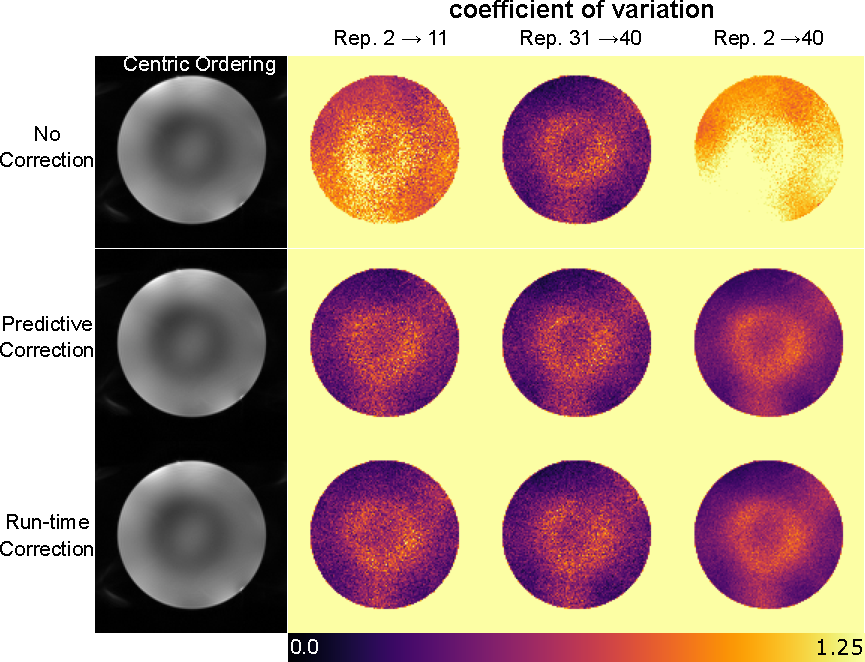
\includegraphics[width=0.8\textwidth]{supporting_information_figures/phantom_drift_result_cnt.pdf}
 \caption{\ A comparison between no RFPA drift correction, predictive RFPA drift correction, and \rev{run}-time RFPA drift correction in a phantom study with centric reordered k-space sampling pattern. The initial repetition is excluded from the analysis to mitigate the impact of the transient
state. The utilization of RFPA correction leads to more uniform CV values similar to the results shown in Figure 5.}
% \label{sif:bssfp_centric}
\end{figure*}


\begin{figure*}
    \centering
    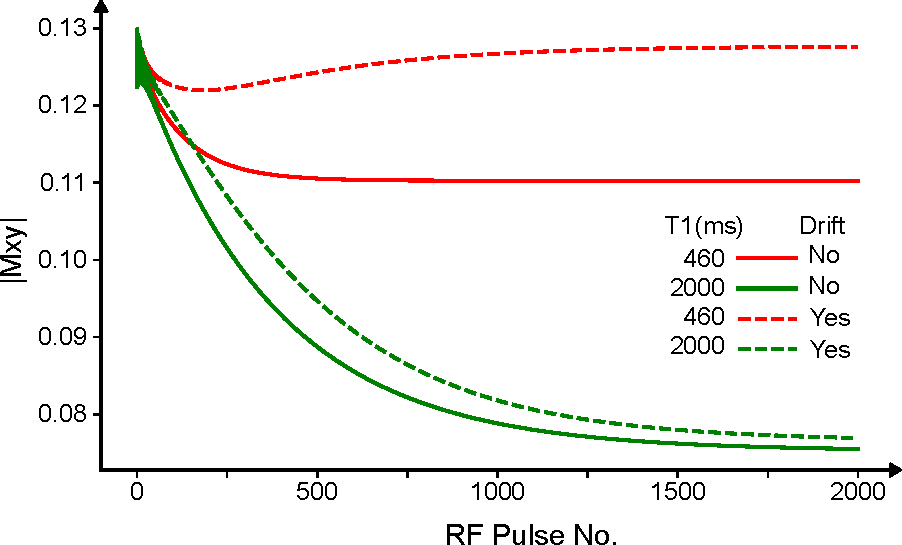
\includegraphics[width=0.7\textwidth]{supporting_information_figures/bSSFP_sim.pdf}
    
    \caption{\ The signal evolution simulation is conducted for a bSSFP sequence by applying a train of preparation pulses using two different $\text{T}_1$ values: 460\,ms and 2000\,ms. The dashed lines of the same color represent the simulation results in the presence of drift. The plotted curves reveal several insights. Firstly, for FA of 15\textdegree, the steady-state signal with a $\text{T}_1$ value of 460\,ms achieves a higher level. Moreover, the signal exhibits a gradual increase and takes more time to reach a steady state. On the other hand, for $\text{T}_1$\,=\,2000\,ms, the discrepancy between the ideal and drifted simulations is significantly smaller compared to the case with $\text{T}_1$\,=\,460\,ms. 
    }
% \label{sif:bssfp_simulation}
\end{figure*}


\begin{figure*}
    \centering
    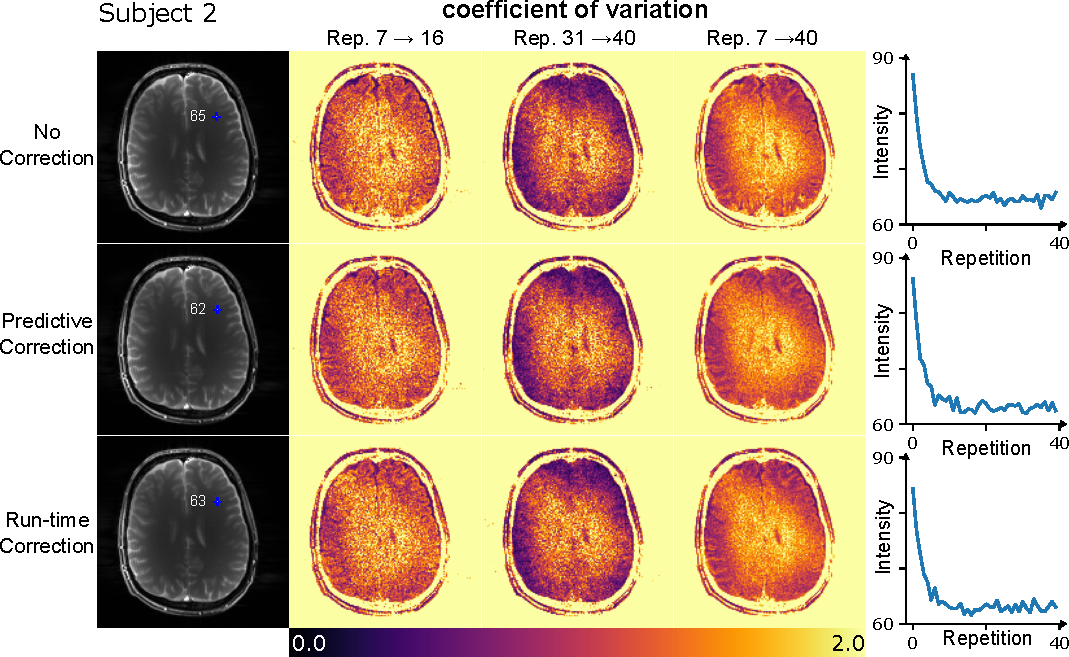
\includegraphics[width=\textwidth]{supporting_information_figures/sub4_drift_result.pdf}
    
    \caption{\ A comparison of CV is presented for the second subject who participated in the study. The analysis includes the scenarios of no RFPA drift correction and the two proposed approaches for drift correction. Similar to the results obtained from subject 1, the first seven repetitions are excluded from the analysis to minimize the contribution of the transient state. However, due to the extended $\text{T}_1$ of GM and WM at 9.4T, the computed CV reflects a combined impact of the transient state and RFPA drift. The last column of the figure illustrates the evolution of voxel intensity, represented by the blue cross in the first column, across all repetitions.
    }
% \label{sif:bssfp_subject4}
\end{figure*}

\begin{figure*}
    \centering
    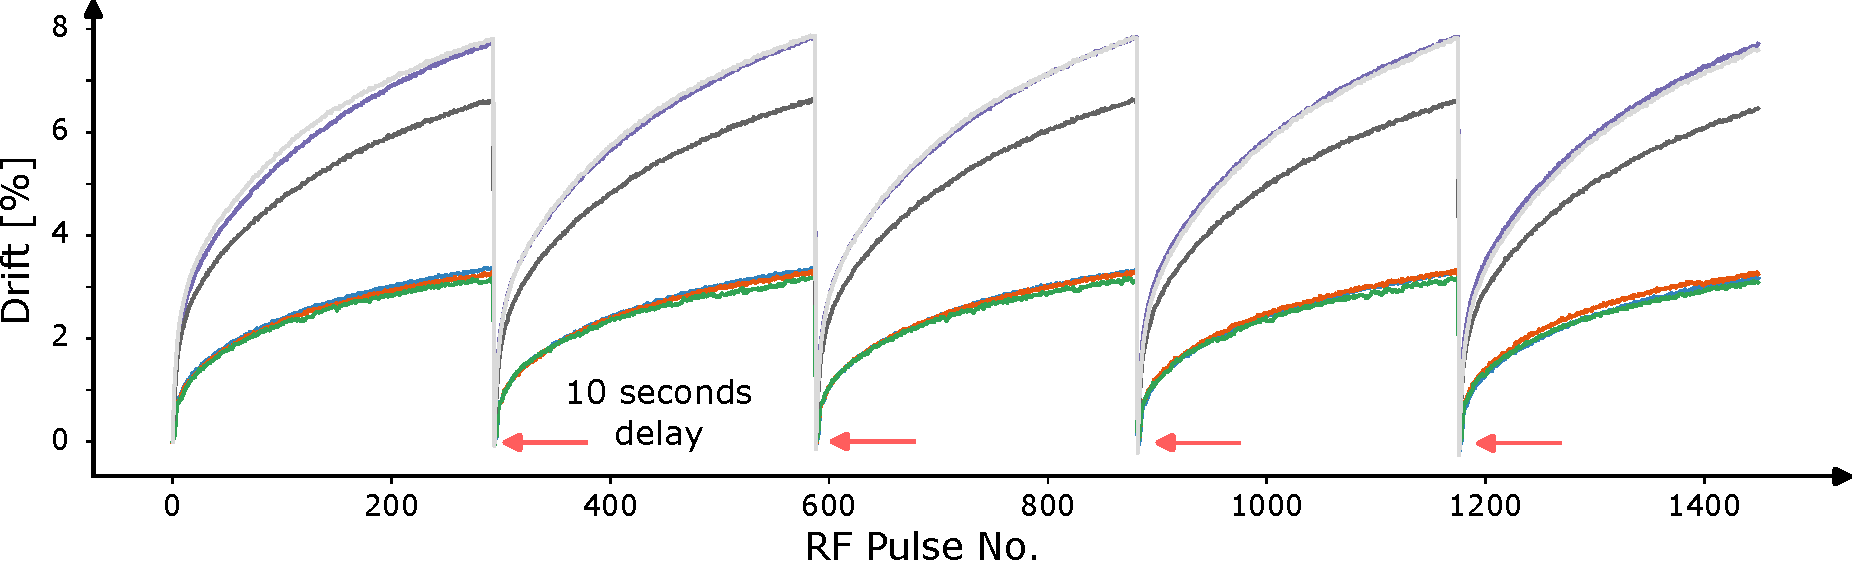
\includegraphics[width=\textwidth]{supporting_information_figures/drift_repeatability.pdf}
    
    \caption{\ \rev{Demonstrating the reproducibility in RFPA drifting magnitude. A single slice is measured using the bSSFP sequence five times (TR=3.5ms, RF=1ms), with a 10-second delay between measurements to enable relaxation of the RFPA. The necessary delay for RFPA relaxation is determined experimentally. Drifting in six exemplary Tx channels is depicted for simplicity. The predictive correction approach is based on the consistency of the drifting curve between calibration and correction scans. It is important to note that potential distortion may occur due to RFPA malfunctions, which are not reproducible.}
    }
% \label{sif:drift_repeatability}    
\end{figure*}

\begin{figure*}
    \centering
    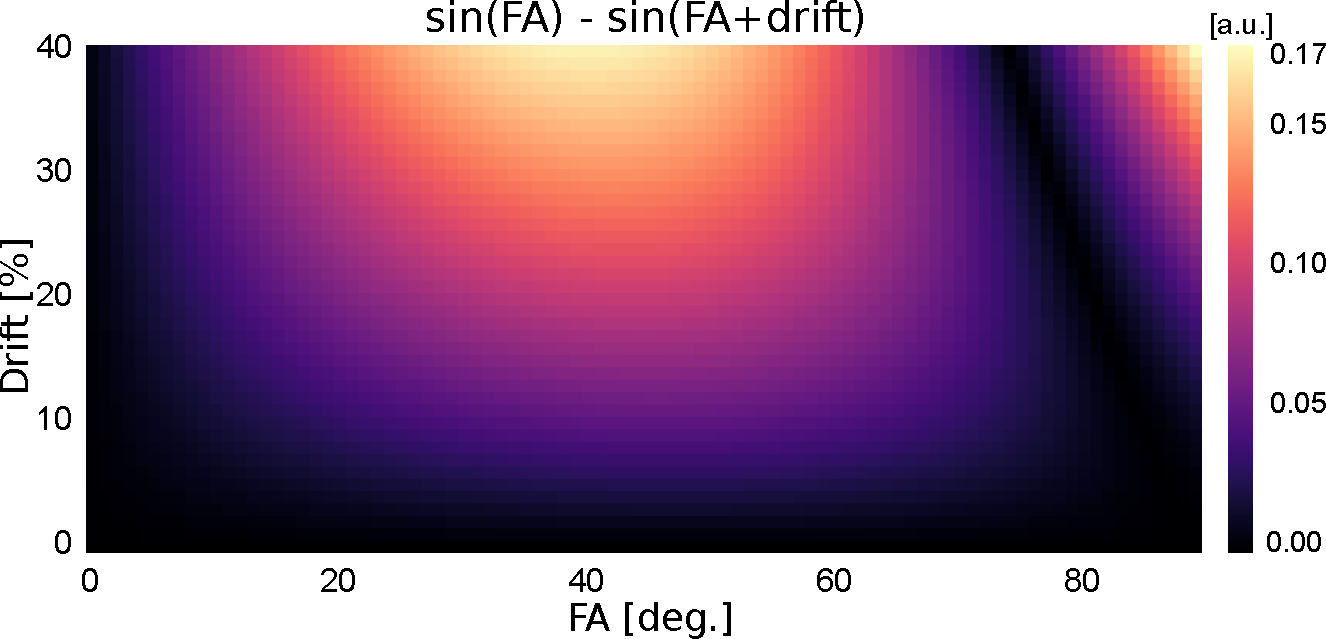
\includegraphics[width=0.8\textwidth]{supporting_information_figures/signal_drift_sensitivity.pdf}
    
    \caption{\ The obtained MR signal originates from the transverse component of magnetization, and its magnitude is correlated to the flip angle (FA) through the sine function. The figure illustrates the discrepancy in the magnitude of the transverse component between the ideal excitation and the drifted excitation for various FA values, considering possible drift effects.
    }
% \label{sif:signal_drift_sensitivity}    
\end{figure*}


\begin{figure*}
    \centering
    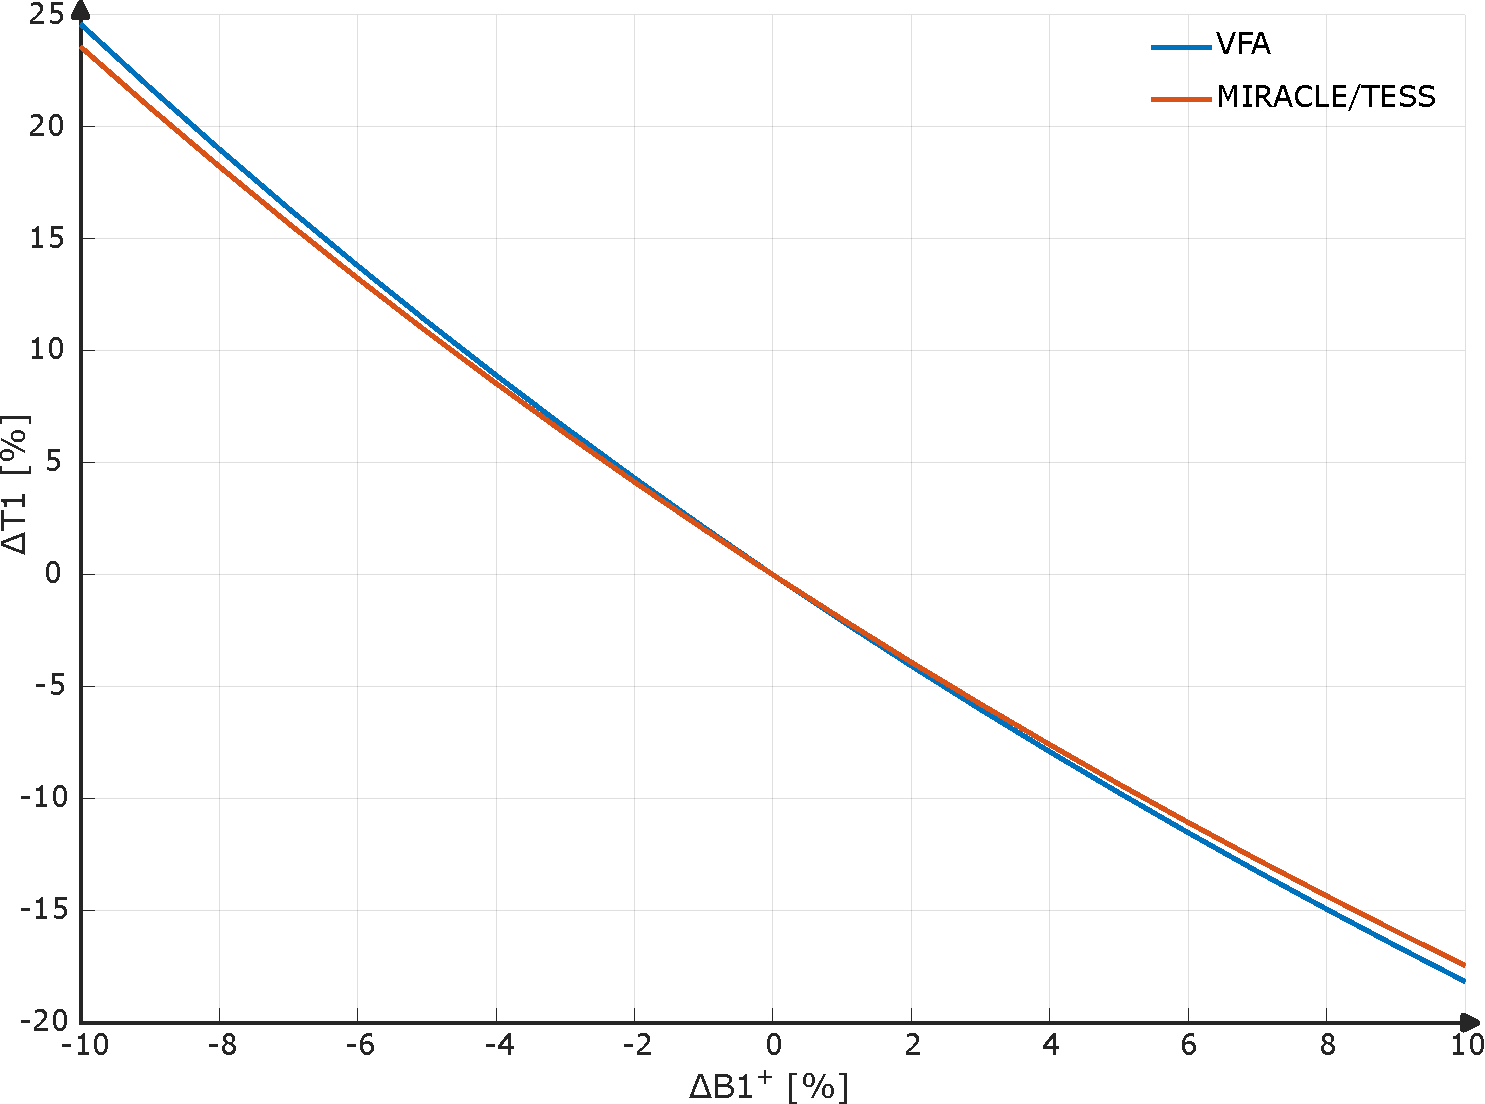
\includegraphics[width=0.8\textwidth]{supporting_information_figures/T1_B1_dep.pdf}
    
    \caption{\ \rev{$\mathrm{T_{1}}$ bias (y axis) resulting from a $\mathrm{B_{1}^{+}}$ quantification error (x axis) for variable flip angle (VFA), motion-insensitive rapid configuration relaxometry (MIRACLE), and triple echo steady state (TESS). Simulation parameters: TR = 5 ms, $\mathrm{T_{1}}$ / $\mathrm{T_{2}}$ = 1425 ms / 29 ms corresponding to WM at 9.4T reported in literature, actual (true) $\mathrm{B_{1}^{+}}$ = 1.0, flip angles: 3°/15° (VFA), 10° (MIRACLE/TESS), RF spoiling increment: 50° (VFA). $\mathrm{B_{1}^{+}}$ and $\mathrm{T_{1}}$ errors were defined as: $\Delta\mathrm{B_{1}^{+}}=((\mathrm{B_{1,est}^{+}}-\mathrm{B_{1,act}^{+}})/\mathrm{B_{1,act}^{+}})\cdot100$, $\Delta\mathrm{T_{1}}=((\mathrm{T_{1,est}}-\mathrm{T_{1,act}})/\mathrm{T_{1,act}})\cdot100$ with estimated (est) and actual/true (act) values. The $\mathrm{B_{1}^{+}}$ error is referring to potential inaccuracies in the employed external $\mathrm{B_{1}^{+}}$ mapping method. MIRACLE and TESS exhibit the same $\mathrm{B_{1}^{+}}$ sensitivity since relaxometry is based on the same signal equations, but different acquisition schemes.}
    }
% \label{sif:T1_B1_dep}    
    
\end{figure*}



\end{document}
